\begin{refsection}

\chapter{Rb--Sr, Sm--Nd, Lu--Hf and Re--Os}\label{ch:PD}

Rb--Sr, Sm--Nd, Lu--Hf and Re--Os all fall in the category of simple
parent-daughter chronometers, which are based on a single parent that
decays to a single daughter without additional complications such as
branched decay or secular equilibrium. These chronometers usually
involve liquid chromatography and mass spectrometry by TIMS or
solution ICP-MS. Data can be introduced into \texttt{IsoplotR} in
three formats:

\begin{enumerate}
\item{`Normal':}
  $\frac{\mbox{P}}{\mbox{d}}$,  
  $\mbox{err}\!\left[\frac{\mbox{P}}{\mbox{d}}\right]$, 
  $\frac{\mbox{D}}{\mbox{d}}$,  
  $\mbox{err}\!\left[\frac{\mbox{D}}{\mbox{d}}\right]$,  
  $\mbox{r}\!\left[\frac{\mbox{P}}{\mbox{d}},
  \frac{\mbox{D}}{\mbox{d}}\right]$
\item{`Inverse':}
  $\frac{\mbox{P}}{\mbox{D}}$,  
  $\mbox{err}\!\left[\frac{\mbox{P}}{\mbox{D}}\right]$, 
  $\frac{\mbox{d}}{\mbox{D}}$,  
  $\mbox{err}\!\left[\frac{\mbox{d}}{\mbox{D}}\right]$,  
  $\mbox{r}\!\left[\frac{\mbox{P}}{\mbox{D}},
  \frac{\mbox{d}}{\mbox{D}}\right]$
\item{`Concentrations':}
  \textbf{P}, err[\textbf{P}], \textbf{D}, err[\textbf{D}], P/D
\end{enumerate}

\noindent where

\noindent P = \textsuperscript{87}Rb, \textsuperscript{147}Sm,
\textsuperscript{187}Re or \textsuperscript{176}Lu.

\noindent D = \textsuperscript{87}Sr, \textsuperscript{143}Nd,
\textsuperscript{187}Os or \textsuperscript{176}Hf.

\noindent d = \textsuperscript{86}Sr, \textsuperscript{144}Nd,
\textsuperscript{188}Os or \textsuperscript{177}Hf.

\noindent \textbf{P} = the elemental concentration (in ppm) of Rb, Sm,
Re, or Lu.

\noindent \textbf{D} = the elemental concentration (in ppm) of Sr, Nd,
Os, or Hf.\\

Format~1 can be converted to format~2 (and vice versa) using
Equation~\ref{eq:format12transformation}, whereas Format~3 can be
converted to format~1 with the methods that were used in
Chapter~\ref{ch:exercises}. For example, for Rb--Sr:
\begin{equation}
  \left({}^{87}\mbox{Rb}/{}^{86}\mbox{Sr}\right) = 
  \frac{\mbox{\textbf{Rb}}}{\mbox{\textbf{Sr}}}
  \frac{\mbox{M(Rb)}}{\mbox{M(Sr)}}
  \frac{
    1+\left[{{}^{87}\mbox{Sr}}/{{}^{86}\mbox{Sr}}\right]
    \left[1+({}^{84}\mbox{Sr}/{}^{87}\mbox{Sr}) +
      ({}^{88}\mbox{Sr}/{}^{87}\mbox{Sr}) \right]
  }{
    1+[{}^{85}\mbox{Rb}/{}^{87}\mbox{Rb}]
  }
  \label{eq:ppm2ratios}
\end{equation}

\noindent where (\textsuperscript{84}Sr/\textsuperscript{87}Sr),
(\textsuperscript{88}Sr/\textsuperscript{87}Sr) and
(\textsuperscript{85}Rb/\textsuperscript{87}Rb) are constant,
non-radiogenic isotope ratios, and M(Rb) and M(Sr) are the molar
masses of Rb and Sr, respectively. Because the measured
(\textsuperscript{87}Sr/\textsuperscript{86}Sr)-ratio appears in
Equation~\ref{eq:ppm2ratios}, the covariance between
\textsuperscript{87}Rb/\textsuperscript{86}Sr and
\textsuperscript{87}Sr/\textsuperscript{86}Sr is nonzero and can be
estimated using Equation~\ref{eq:s2t} or \ref{eq:s2tmatrix}.\\

The parent-daughter pair methods are generally used to form
multi-aliquot isochrons that can either be plotted in conventional or
inverse isochron space. For the U--Pb, Ar--Ar, Pb--Pb and K-Ca
methods, the nonradiogenic daughter isotope is less abundant than the
radiogenic isotope. However this is not the case for the Rb--Sr,
Sm--Nd, Re--Os and Lu--Hf methods. Their non-radiogenic isotopes
(marked as `d' above) tend to be more abundant than the radiogenic
isotope and they therefore exhibit weaker error correlations in
conventional isotope space. Nevertheless, \texttt{IsoplotR} does offer
the inverse isochron as an option because it is may still be useful to
visualise the data as a simple mixing line between non-radiogenic and
radiogenic components.\\

\noindent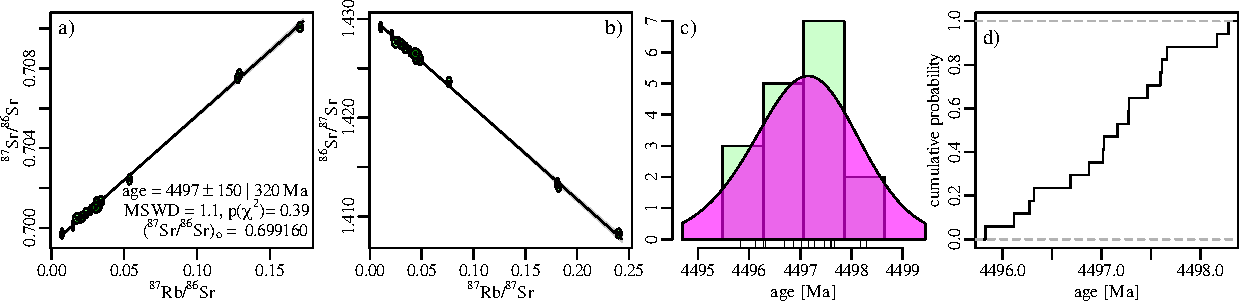
\includegraphics[width=\textwidth]{../figures/RbSr.pdf}
\begingroup\captionof{figure}{a) conventional and b) inverse Rb--Sr
  isochron, c) KDE and d) CAD of the single aliquot age estimates
  using the isochron intercept as a non-radiogenic
  \textsuperscript{87}Sr/\textsuperscript{86}Sr-ratio.\\}
\label{fig:RbSrabcd}\endgroup

The distribution of the data around the best fit isochron can be
visually assessed on radial plots, KDEs and CADs. This is achieved by
projecting the data along parallel lines to the best fit in inverse
isochron space as in
Figure~\ref{fig:ThPbSingleGrain}.a. Alternatively, the assumption of
cogenetic origin may be relaxed by fixing the non-radiogenic
composition and computing two-point isochrons between this composition
and the measured ratios for each aliquot
(Figure~\ref{fig:ThPbSingleGrain}.b).

\printbibliography[heading=subbibliography]

\end{refsection}
